\documentclass[a4paper,12pt]{report}
\usepackage[utf8]{vietnam}
\usepackage{graphicx}
\usepackage{fancybox}
\usepackage{longtable}
\usepackage{listings}
\usepackage[left=3cm, right=2.00cm, top=2.00cm, bottom=2.00cm]{geometry}
\lstset{
   %keywords={break,case,catch,continue,else,elseif,end,for,function,
   %   global,if,otherwise,persistent,return,switch,try,while},
   basicstyle=\ttfamily \fontsize{12}{15}\selectfont,   
	% numbers=left,
   frame=lrtb,
tabsize=3
}
\PassOptionsToPackage{hyphens}{url}\usepackage{hyperref}  
\usepackage{float}
\hypersetup{
    colorlinks,
    citecolor=black,
    filecolor=black,
    linkcolor=black,
    urlcolor=black
}
\setlength{\parskip}{0.6em}
\usepackage[nottoc]{tocbibind}
\usepackage[english]{babel}
\addto\captionsenglish{%
 \renewcommand\chaptername{Phần}
 \renewcommand{\contentsname}{Mục lục} 
 \renewcommand{\listtablename}{Danh sách bảng}
 \renewcommand{\listfigurename}{Danh sách hình vẽ}
 \renewcommand{\tablename}{Bảng}
 \renewcommand{\figurename}{Hình}
 \renewcommand{\bibname}{Tài liệu tham khảo}
}

\begin{document}
\thispagestyle{empty}
\thisfancypage{
\setlength{\fboxrule}{1pt}
\doublebox}{}
\begin{center}
{\fontsize{16}{19}\fontfamily{cmr}\selectfont TRƯỜNG ĐẠI HỌC BÁCH KHOA HÀ NỘI\\
VIỆN CÔNG NGHỆ THÔNG TIN VÀ TRUYỀN THÔNG}\\
\textbf{------------*******---------------}\\[1cm]

\includegraphics[scale=0.13]{hust.jpg}\\[1.3cm]

{\fontsize{32}{43}\fontfamily{cmr}\selectfont BÁO CÁO}\\[0.1cm]
{\fontsize{38}{45}\fontfamily{cmr}\fontseries{b}\selectfont MÔN HỌC}\\[0.2cm]
{\fontsize{19}{20}\fontfamily{phv}\selectfont Xử lý ngôn ngữ tự nhiên}\\[0.2cm]
{\fontsize{13}{20}\fontfamily{cmr}\selectfont \emph{Đề tài: Phân tích quan điểm}}\\[2.5cm]
\end{center}
\hspace{1.5cm}\fontsize{14}{16}\fontfamily{cmr}\selectfont \textbf{Nhóm sinh viên thực hiện:}

\begin{longtable}{l c c}

Họ và tên & MSSV  & Lớp\\

Nguyễn Tuấn Đạt & 20130856 & CNTT2.02-K58 \\
Phan Anh Tú &   20134501 & CNTT2.01-K58\\

\end{longtable}

\hspace{1cm}\fontsize{14}{16}\fontfamily{cmr}\selectfont \textbf{Giáo viên hướng dẫn: }PGS.TS Lê Thanh Hương \\[2cm]
\begin{center}
\fontsize{16}{19}\fontfamily{cmr}\selectfont Hà Nội 12--2016

\end{center}
\newpage
\tableofcontents
\listoftables
\listoffigures

\chapter*{Lời cảm ơn}
\phantomsection
\addcontentsline{toc}{chapter}{Lời cảm ơn}
Đề tài sẽ không thể hoàn thành nếu không nhờ có sự tận tình chỉ bảo và hướng dẫn của cô giáo PGS.TS Lê Thanh Hương. Mặc dù đã rất cố gắng để hoàn thành tốt nhưng trong quá trình làm việc, sai sót là điều không thể tránh khỏi. Nhóm chúng em mong nhận được nhận xét và phê bình của quý thầy cô để đề tài được hoàn thiện hơn đồng thời bổ sung những kiến thức còn thiếu sót cho chúng em.


Chúng em xin chân thành cảm ơn!

\chapter{Đặt vấn đề }
Cùng với sự phát triển mạnh mẽ của ngành công nghệ thông tin và truyền thông, trí tuệ nhân tạo đang ngày càng phát triển và có thể nói trong tương lai không xa máy tính sẽ trở nên thông minh chẳng kém gì con người. Trong trí tuệ nhân tạo thì hai mảng học máy và xử lý ngôn ngữ tự nhiên là hai mảng tiềm năng và phát triển cực mạnh, là hai trong số rất nhiều mảng của trí tuệ nhân tạo được tập trung nghiên cứu nhiều nhất hiện nay.


Là những sinh viên ngành công nghệ thông tin, là một kỹ sư công nghệ thông tin trong tương lai, chúng em nhận thấy cần phải trang bị cho mình những kiến thức nền tảng và những kinh nghiệm trong các bài toán thực tế về các mảng xử lý ngôn ngữ tự nhiên và học máy. Vì vậy, mục tiêu của bài tập lớn môn học này của chúng em là tìm hiểu lý thuyết và ứng dụng các kỹ thuật học máy cụ thể là hai phương pháp: \textbf{Support Vector Machine (SVM)} và \textbf{Deep Learning} (\textbf{Long Short Term Memory (LSTM)}) vào bài toán phân tích quan điểm của mảng xử lý ngôn ngữ tự nhiên.


Các nội dung triển khai trong đề tài này được thực hiện theo nhóm gồm hai sinh viên bao gồm: Nguyễn Tuấn Đạt và Phan Anh Tú. Trong đó dưới sự hướng dẫn của cô giáo PGS.TS Lê Thanh Hương, mỗi người phụ trách một số nội dung tách biệt nhau:
\begin{enumerate}
\item Nguyễn Tuấn Đạt
\begin{itemize}
\item Tìm hiểu và cài đặt SVM
\end{itemize}
\item Phan Anh Tú
\begin{itemize}
\item Tìm hiểu và cài đặt RNN,LSTM
\end{itemize}
\end{enumerate}
Phần tiếp theo của báo cáo bao gồm các phần sau:
\par Phần 2: Trình bày tóm lược về lý thuyết cách biểu diễn dữ liệu; các phương pháp học máy áp dụng: SVM, RNN-LSTM


\chapter{Cơ sở lý thuyết}
\section{Biểu diễn dữ liệu}
\subsection{One-hot vector}
\section{SVM}
\section{Recurrent Neural Network (RNN)}
\subsection{RNN}
Recurrent Neural Network (RNN) là một mô hình phổ biến trong nhiều bài toán liên quan đến xử lý ngôn ngữ tự nhiên. Ý tưởng của RNN là sử dụng các thông tin liên tục (ghi nhớ các thông tin đã xử lý ở quá khứ). Sở dĩ RNN thích hợp cho bài toán xử lý ngông ngữ tự nhiên do ở mạng neuron truyền thống chúng ta giả sử tất cả các input sẽ được xử lý độc lập và đưa ra các output cũng độc lập với nhau. Mà các bài toán xử lý ngôn ngữ tự nhiên thì làm việc với đầu vào là các câu, các văn bản và mỗi câu trong văn bản hay mỗi từ trong một câu thì thường là không độc lập với nhau, chúng có mỗi liên hệ với nhau. Ví dụ với bài toán đoán từ tiếp theo trong câu thì để đoán được từ tiếp theo thì ta cần dựa vào các từ trước đó. Để giải quyết vấn đề đó, RNN sẽ xử lý các input theo thứ tự và đưa ra các output phụ thuộc vào các tính toán trước đó, hay nói cách khác RNN sẽ nhớ các thông tin trong quá khứ đã xử lý.
\par Mạng RNN có thể mô tả như hình vẽ dưới đây: 
\begin{figure}[H]
\centering
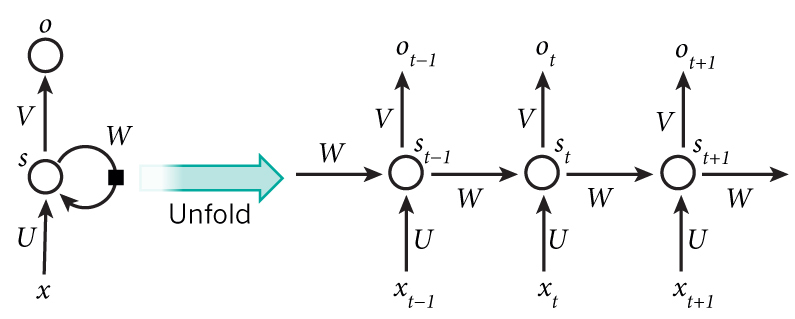
\includegraphics[scale=0.5]{rnn.jpg}
\caption{Mạng RNN}
\label{img_rnn}
\end{figure}
Trong hình \ref{img_rnn}:
\begin{itemize}
\item $x_t$ là input tại thời điểm t. Ví dụ: $x_0, x_1, x_2$ là one-hot vector của các từ 1, 2, 3 đầu vào.
\item $s_t$ là một trạng thái ẩn (trạng thái tạm thời, thông tin ghi nhớ). $s_t$ được tính phụ thuộc vào trạng thái ẩn phía trước và input của thời điểm hiện tại. $s_t = f(Ux_t + Ws_{t-1})$. Hàm f thường là hàm phi tuyến như \textbf{tanh} hoặc \textbf{ReLU}. $s_{-1}$ là đầu vào khi tính $s_0$ (trạng thái tạm thời đầu tiên), $s_{-1}$ thường bằng 0.
\item $o_t$ là output tại thời điểm t. Ví dụ: Nếu ta muốn đoán từ tiếp theo trong câu, $o_t$ là vector xác suất của các từ trong từ điển (nếu đầu vào là one-hot vector). $o_t = softmax(Vs_t)$
\end{itemize}
Các điều cần chú ý:
\begin{itemize}
\item Các bước tính toán sẽ được tính lần lượt. Ví dụ input đầu vào là một câu có 5 từ ($x_0, x_1, x_2, x_3, x_4$). Thì sau khi tính ra trạng thái ẩn ($s_0$) của từ thứ nhất ($x_0$) thì mới sử dụng thông tin $s_0, x_1$ để tính $s_1$. Các output $o_t$ có thể đưa ra hoặc không đưa ra ở mỗi bước tuỳ vào bài toán cụ thể: ví dụ ở bài toán phân tích quan điểm của một câu, ta chỉ cần đưa ra output cuối cùng (quan điểm của cả câu) mà không cần đưa ra các output ở mỗi bước (quan điểm của mỗi từ trong câu). Đặc trưng của RNN là các trạng thái ẩn, nơi mà giữ thông tin của các bước trước đó.  
\item Các trạng thái ẩn $s_t$ như là bộ nhớ (memory) của mạng RNN. $s_t$ sẽ giữ lại thông tin của các thời điểm phía trước. Output $o_t$ được tính toán dựa vào các thông tin đã ghi nhớ được tại thời điểm t.
\item Nếu như ở mạng neural truyền thống, mỗi tầng sẽ sử dụng các tham số khác nhau, thì ở RNN sẽ chia sẻ các tham số (U,W,V) ở tất cả các bước.
\end{itemize}

\subsubsection{Vấn đề Long-Term Dependencies}
Vấn đề  Long-Term Dependencies là vấn đề: trong xử lý tại bước hiện tại ta cần quá nhiều thông tin phụ thuộc không cần thiết của các bước trước.Một trong những đặc điểm nổi bật của RNN là mô hình này sẽ kết nối những thông tin phía trước để hỗ trợ cho bước xử lý hiện tại. Nhưng đôi khi ta chỉ cần dựa vào một số thông tin gần nhất để thực hiện bước xử lý hiện tại. Ví dụ trong bài toán đoán từ tiếp theo (\emph{sky}) trong đoạn văn có câu \emph{the clouds are in the sky} ta không cần những thông tin của quá nhiều từ trước đó ta vẫn có thể đoán được. Trong trường hợp này, khoảng cách tới cách thông tin liên quan được rút ngắn lại. Theo như mô hình chuẩn của RNN thì tất cả các thông tin của các bước phía trước đều được ghi nhớ lại và cung cấp cho bước xử lý hiện tại, dẫn đến việc dư thừa, không cần thiết. Vì vậy, mạng LSTM (Long Short Term Memory) đã xuất hiện để giải quyết vấn đề này.

\subsection{LSTM}
\subsubsection{Giới thiệu LSTM}
Mạng LSTM là một dạng đặc biệt của mạng RNN. LSTM được thiết kế để khắc phục vấn đề Long-Term Dependencies của RNN. 
\par Mô hình RNN chuẩn là việc lặp lại các module, các module này có cấu trúc đơn giản chỉ gồm một \textbf{tanh layer}.
\begin{figure}[H]
\centering
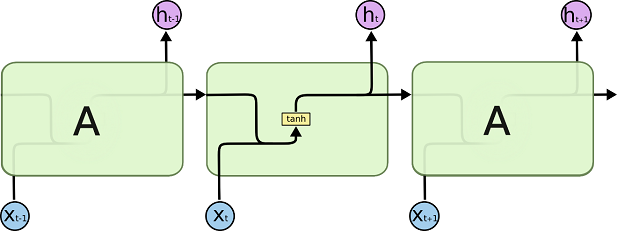
\includegraphics[scale=0.7]{rnn_tanh.jpg}
\caption{Mô hình RNN chuẩn với hàm tanh}
\end{figure}
\par LSTM cũng có cấu trúc lặp tương tự nhưng các module lặp có cấu trúc khác. Thay vì chỉ có một \textbf{tanh layer}, ta có bốn layer tương tác với nhau. 
\begin{figure}[H]
\centering
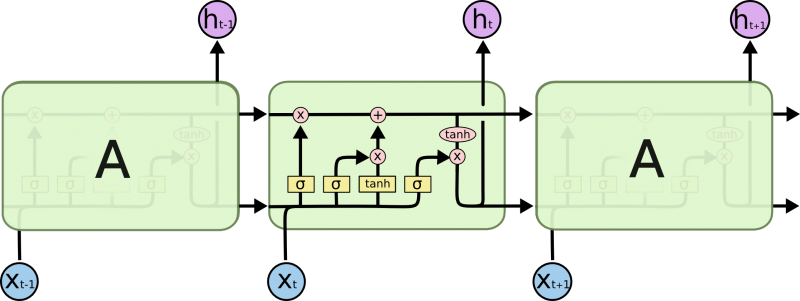
\includegraphics[scale=0.4]{lstm.png}
\caption{Mô hình LSTM}
\end{figure} 

\subsubsection{Ý tưởng chính của LSTM}
Điểm khác biệt lớn nhất của LSTM với RNN, đặc điểm nổi bật của LSTM chính là \textbf{cell state}	



\chapter{Bài toán áp dụng}


\chapter{Kết luận} 
\begin{thebibliography}{9}
\bibitem{1} \url{http://www.wildml.com/2015/09/recurrent-neural-networks-tutorial-part-1-introduction-to-rnns/}
\bibitem{2} \url{http://colah.github.io/posts/2015-08-Understanding-LSTMs/}
\bibitem{3} \url{http://cs224d.stanford.edu/syllabus.html}
\end{thebibliography}


\end{document}
